\section{Exercises}

%%%%%%%%%%%%%%%%%%%

\subsection{Small sample inference for the mean}

%%%%%%%%%%%%%%%%%%%

% 1

\eoce{An independent random sample is selected from an approximately normal population with unknown standard deviation. The sample is small ($n < 50$). Find the degrees of freedom and the critical $t$ value (t$^\star$) for the given confidence level. \vspace{-3mm}
\begin{multicols}{2}
\begin{enumerate}[(a)]
\setlength{\itemsep}{0mm}
\item $n = 42$, CL = 90\%
\item $n = 21$, CL = 98\%
\item $n = 29$, CL = 95\%
\item $n = 12$, CL = 99\%
\end{enumerate}
\end{multicols}
}
{
\begin{enumerate}[(a)]
\setlength{\itemsep}{0mm}
\item $n = 42$, CL = 90\%, $df = 42 - 1 = 41$, $t^{\star}_{41} = 1.68$
\item $n = 21$, CL = 80\%, $df = 21 - 1 = 20$, $t^{\star}_{20} = 2.53$
\item $n = 29$, CL = 95\%, $df = 29 - 1 = 28$, $t^{\star}_{28} = 2.05$
\item $n = 12$, CL = 99\%, $df = 12 - 1 = 11$, $t^{\star}_{11} = 3.11$
\end{enumerate}
}

% 2

{\eoce{A 90\% confidence interval for a population mean is (65,77). The population distribution is approximately normal and the population standard deviation is unknown. Given that this confidence interval is calculated based on an independent random sample of size 25, calculate the sample mean, the margin of error, and the sample standard deviation.
}
{
The sample mean is the midpoint of the confidence interval: $\bar{x} = \frac{65 + 77}{2} = 71$ \\
The margin of error is half the width of the confidence interval: $ME = \frac{77 - 65}{2} = 6$ \\
Using $df = 25 - 1 = 24$ and the confidence level of 90\% we can find the critical value from the t-table: $t^{\star}_{24} = 1.71$. Lastly, using the margin of error and the critical value we can solve for $s$:
\begin{align*}
ME &= t^{\star}_{24} \frac{s}{\sqrt{n}} \\
6 &= 1.71 \frac{s}{\sqrt{25}} \\
&= 0.342 s \\
s &= 17.54
\end{align*}
}
}

% 3

\eoce{For a given confidence level, $t^{\star}_{df}$ is larger than $z^{\star}$. Explain how $t^{*}_{df}$ being slightly larger than $z^{*}$ affects the width of the confidence interval.}
{
With a larger critical value, the confidence interval ends up being wider. This makes intuitive sense as when we have a small sample size and the population standard deviation is unknown, we should have a wider interval than if we knew the population standard deviation, or if we had a large enough sample size.
}

% 4

\eoce{An independent random sample is selected from an approximately normal population with unknown standard deviation. The sample is small ($n < 50$). Find the p-value for the given set of hypotheses and $t$ values. Also determine if the null hypothesis would be rejected at $\alpha = 0.05$. \vspace{-3mm}
\begin{multicols}{2}
\begin{enumerate}[(a)]
\setlength{\itemsep}{0mm}
\item $H_A: \mu > \mu_0 $, $n = 11$, $T = 1.91$
\item $H_A: \mu < \mu_0 $, $n = 17$, $T = -3.45$
\item $H_A: \mu \ne \mu_0 $, $n = 38$, $T = 0.83$
\item $H_A: \mu > \mu_0 $, $n = 47$, $T = 2.13$
\end{enumerate}
\end{multicols}
}
{
\begin{enumerate}[(a)]
\setlength{\itemsep}{0mm}
\item $H_A: \mu > \mu_0 $, $n = 11$, $T= 1.91$, $df = 11 - 1 = 10$, $0.025 < p-value < 0.05$, Reject $H_0$
\item $H_A: \mu < \mu_0 $, $n = 17$, $T = -3.45$, $df = 17 - 1 = 16$, $p-value < 0.005$, Reject $H_0$
\item $H_A: \mu \ne \mu_0 $, $n = 38$, $T = 0.83$, $df = 38 - 1 = 37$, $p-value > 0.20$, Fail to reject $H_0$
\item $H_A: \mu > \mu_0 $, $n = 47$, $T = 2.13$, $df = 47 - 1 = 46$, $0.01 < p-value < 0.025$, Reject $H_0$ \\
\end{enumerate}

\begin{center}
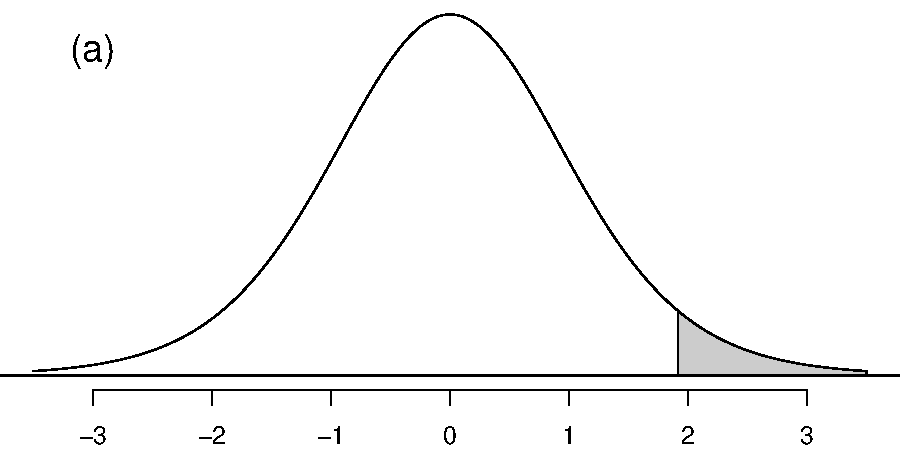
\includegraphics[width=55mm]{06/figures/eoce/oneSampleTa.pdf}
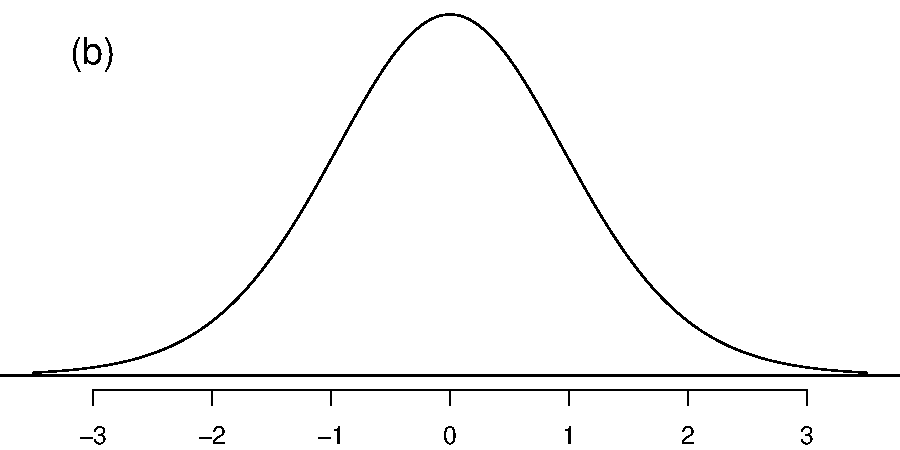
\includegraphics[width=55mm]{06/figures/eoce/oneSampleTb.pdf} \\
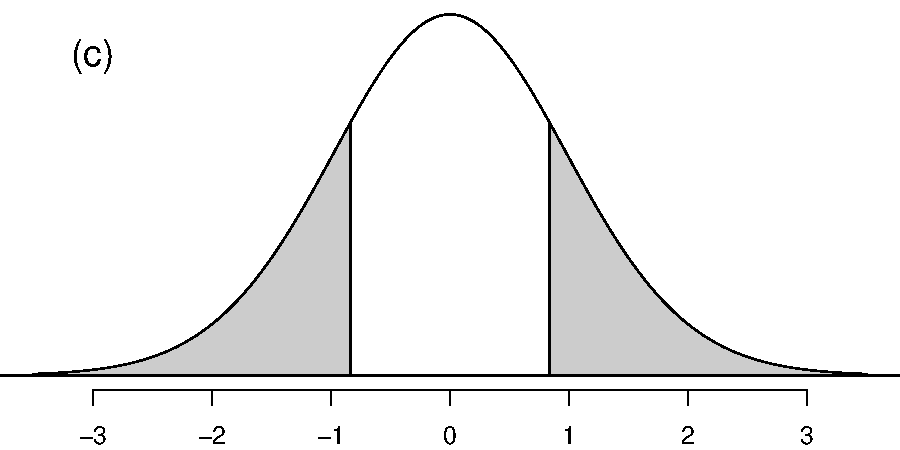
\includegraphics[width=55mm]{06/figures/eoce/oneSampleTc.pdf}
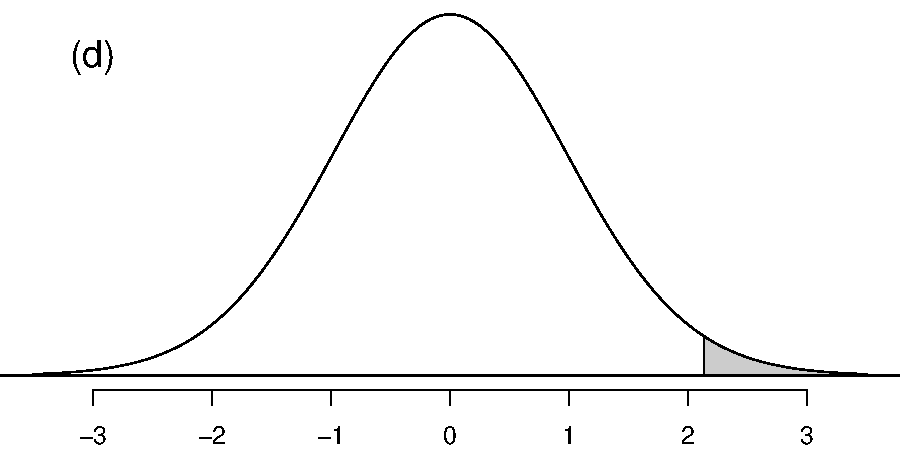
\includegraphics[width=55mm]{06/figures/eoce/oneSampleTd.pdf}
\end{center}
}

% 5

\eoce{
New York is known as ``the city that never sleeps". A random sample of 25 New Yorkers were asked how much sleep they get per night. A summary of some sample statistics is shown below. Do these data provide strong evidence that New Yorkers on average sleep less than 8 hours a night?
\begin{center}
\begin{tabular}{rrrrrr}
 \hline
n 	& $\bar{x}$	& s		& min 	& max \\ 
 \hline
25 	& 7.73 		& 0.77 	& 6.17 	& 9.78 \\ 
  \hline
\end{tabular}
\end{center}

\begin{enumerate}[(a)]
\setlength{\itemsep}{0mm}
\item Write the hypotheses in symbols and in words.
\item Calculate the test statistic, $T$. (Reminder: check conditions and assumptions.)
\item Find and interpret the p-value in context. Drawing a picture may be helpful.
\item What is the conclusion of the hypothesis test?
\item If you were to construct a confidence interval that corresponded to this hypothesis test, would you expect 8 hours to be in the interval?
\end{enumerate}
}
{
\begin{enumerate}[(a)]
\setlength{\itemsep}{0mm}

\item $H_0: \mu = 8$ (New Yorkers on average sleep 8 hrs per night.) \\
$H_A: \mu < 8$ (New Yorkers on average sleep less than 8 hrs per night.)

\item Before calculating the test statistic we should check that the assumptions and conditions are satisfied.
\begin{enumerate}[1.]
\item Independence Assumption: 
\begin{itemize}
\item Random Sampling Condition: We are told that the sample is random.
\item 10\% Condition: 25 $<$ 10\% of all New Yorkers.
\end{itemize}
Since we have a random sample and the 10\% condition is satisfied, we can assume that the number of hours one New Yorker in the sample sleeps is independent of another.
\item Nearly Normal Condition: We do not have a plot of the data however we can tell that there are no extreme outliers as all observations are within 2 standard deviations of the mean.
\[ 7.73 \pm 2 * 0.77 = (6.18, 9.26) \]
If there is skew, it is not strong. There are no red flags for the normal model based on this (limited) information, and we do not have reason to believe the number of hours New Yorkers sleep per day is not nearly normal. 
\end{enumerate}

The test statistic can be calculated as follows.
\begin{align*}
T &= \frac{\bar{x} - \mu_0}{\frac{s}{\sqrt{n}}} = \frac{7.73 - 8}{\frac{0.77}{\sqrt{25}}} = -1.75\\
df &= 25 - 1 = 24
\end{align*}

\item $0.025 < p-value < 0.05$

\begin{minipage}[c]{0.5\textwidth}
If in fact the true population mean of the amount New Yorkers sleep per night was 8 hours, the probability of getting a random sample of 25 New Yorkers where the average amount of sleep is 7.73 hrs per night or less is between 0.025 and 0.05.
\end{minipage}
\begin{minipage}[c]{0.5\textwidth}
\begin{center}
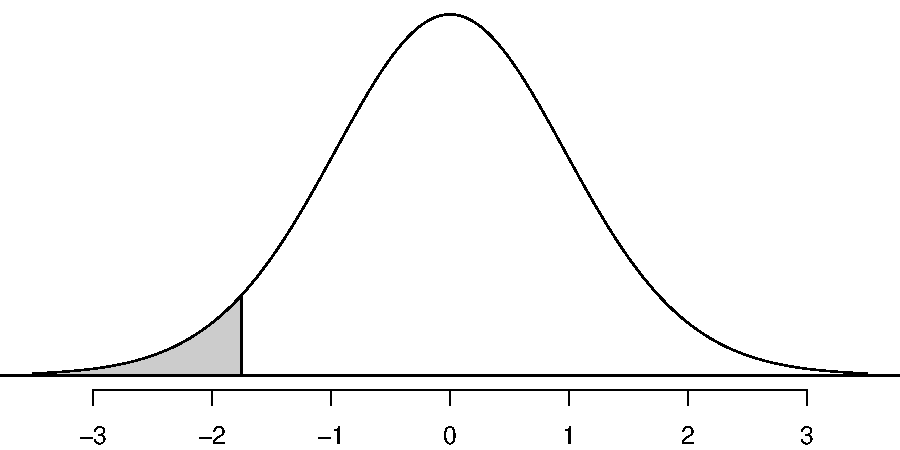
\includegraphics[width=55mm]{06/figures/eoce/newYork.pdf}
\end{center}
\end{minipage}


\item Since p-value $< \alpha$ (use $\alpha = 0.05$ since not given) we reject the null hypothesis. The data provide strong evidence that New Yorkers on average sleep less than 8 hours per night.

\item No, the hypothesis test suggests that the average amount of sleep New Yorkers get is significantly lower than 8 hours per night, therefore we wouldn't expect 8 hours to be in the interval.

\end{enumerate}
}\label{NewYorkSleep}

% 6

\eoce{A college newspaper article claims that students at this college spend more than an hour per day on average on social networking sites. The article is based on a survey conducted at this college on a random sample of 45 college students who use social networking sites, which yielded a sample mean of 68.2 minutes with a standard deviation of 21 minutes. A histogram of the data is shown below. Do these data provide strong evidence that students at this college who use social networking sites spend on average more than an hour (60 minutes) per day on such sites? \vspace{1mm} \\
\noindent \begin{minipage}[c]{0.55\textwidth}
\begin{enumerate}[(a)]
\setlength{\itemsep}{0mm}
\item Write the hypotheses in symbols and in words.
\item Calculate the test statistic, $T$. (Reminder: check conditions and assumptions.)
\item Find and interpret the p-value in context. Drawing a picture may be helpful.
\item What is the conclusion of the hypothesis test?
\item If you were to construct a confidence interval that corresponded to this hypothesis test, would you expect 60 minutes to be in the interval?
\end{enumerate}
\end{minipage}
\begin{minipage}[c]{0.45\textwidth}
\begin{center}
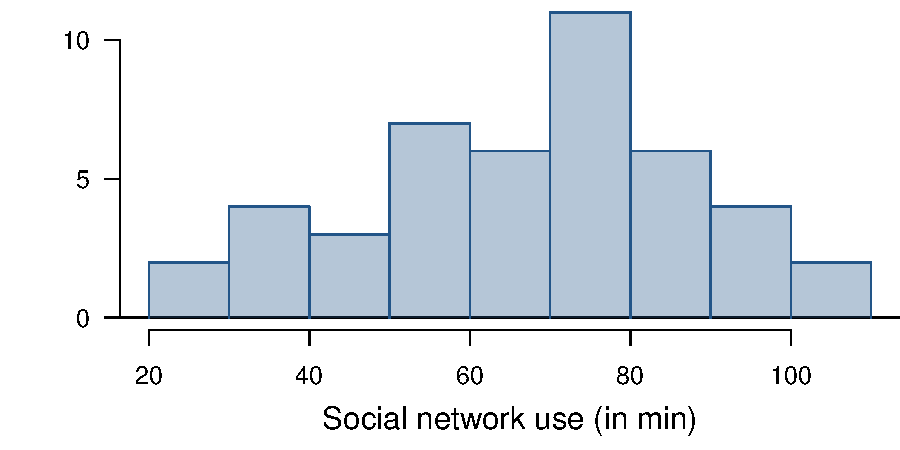
\includegraphics[width= \textwidth]{06/figures/eoce/socNetUseHist}
\end{center}
\end{minipage}
}
{
\begin{enumerate}[(a)]
\setlength{\itemsep}{0mm}
\item $H_0: \mu = 60$ (Students spend an hour per day on average on social networking sites.) \\
$H_A: \mu > 60$ (Students spend more than an hour per day on average on social networking sites.)
\item Before calculating the test statistic we should check that the assumptions and conditions are satisfied.
\begin{enumerate}[1.]
\item Independence Assumption: 
\begin{itemize}
\item Random Sampling Condition: We are told that the sample is random.
\item 10\% Condition: It is safe to assume that 45 $<$ 10\% of all students at this college.
\end{itemize}
Since we have a random sample and the 10\% condition is satisfied, we can assume that the amount of time one student in this sample spends on social networking sites is independent of another.
\item Nearly Normal Condition: The histogram does not show an extremely skewed distribution, therefore we can assume that the amount of time college students spend on social networking sites has an approximately normal distribution.
\end{enumerate}

The test statistic can be calculated as follows.
\begin{align*}
T &= \frac{\bar{x} - \mu_0}{\frac{s}{\sqrt{n}}} = \frac{68.2 - 60}{\frac{20}{\sqrt{45}}} = 2.75\\
df &= 45 - 1 = 44
\end{align*}
\item $p-value < 0.005$ \\
\begin{minipage}[c]{0.5\textwidth}
If in fact students at this college spend on average an hour per day on social networking sites, the probability of getting a random sample of 45 students where the average amount of time spend on social networking sites is 68.2 minutes or higher is less than 0.005.
\end{minipage}
\begin{minipage}[c]{0.5\textwidth}
\begin{center}
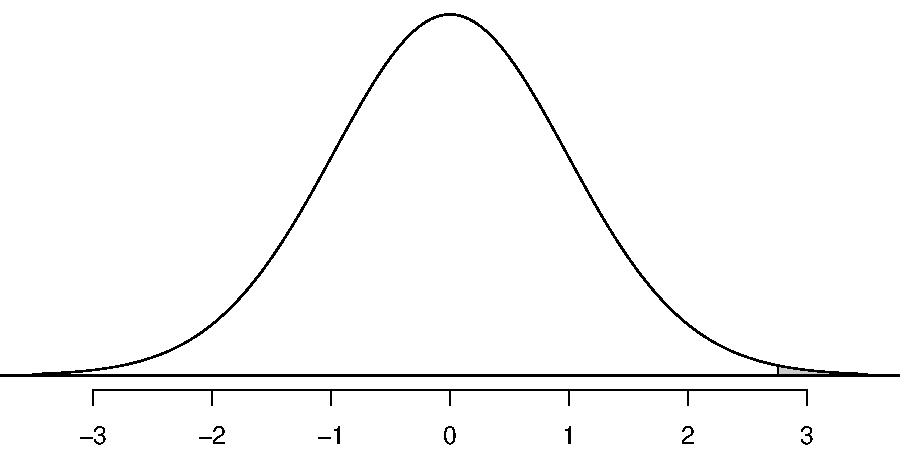
\includegraphics[width=55mm]{06/figures/eoce/socNetUse}
\end{center}
\end{minipage}
\item No, the hypothesis test suggests that the average amount of time students at this college spend on social networking sites per day is significantly higher than 60 minutes, therefore we wouldn't expect 60 minutes to be in the interval.
\end{enumerate}
}\label{socNetUse}

% 7

\eoce{Exercise~\eoceref{NewYorkSleep} provides summary statistics on the number of hours of sleep 25 randomly sampled New Yorkers get per night. 
\begin{enumerate}[(a)]
\setlength{\itemsep}{0mm}
\item Calculate a 90\% confidence interval for the number of hours of New Yorkers sleep on average and interpret this interval in context.
\item Using your confidence interval, would you reject the notion that New Yorkers sleep an average of 8 hours per night?
\end{enumerate}
}
{
\begin{enumerate}[(a)]
\setlength{\itemsep}{0mm}
\item Before we can calculate the confidence interval, we need to find the degrees of freedom and $t^{\star}_{df}$.
\[ df = 25 - 1 = 24 \hspace{5mm} t^{\star}_{df} = 1.71\]

A 90\% confidence interval can be calculated as follows:
\begin{align*}
\bar{x} \pm t^{\star}_{df} \frac{s}{\sqrt{n}} &= 7.73 \pm 1.71\frac{0.77}{\sqrt{25}} \\
&= 7.73 \pm 0.26 \\
&= (7.47, 7.99)
\end{align*}
We are 90\% confident that New Yorkers on average sleep 7.46 to 7.99 hours per night.

\item Yes, since 8 hours is not in the interval we would reject his notion. It should be noted however that the upper bound of the interval is very close to 8. 

\end{enumerate}

}

% 8

\eoce{Exercise~\eoceref{socNetUse} provides the mean (68.2 minutes) and standard deviation (21 minutes) for the time spent on social networking sites of 45 randomly sampled students (under the condition that they use social networking sites) at an unnamed college
\begin{enumerate}[(a)]
\setlength{\itemsep}{0mm}
\item Calculate a 90\% confidence interval for the true average amount of time students at this college spend on social networking sites per day.
\item Using your confidence interval, would you reject the notion that students at this college who use social networking sites spend an average of 60 minutes on these sites?
\end{enumerate}
}
{
\begin{enumerate}[(a)]
\setlength{\itemsep}{0mm}
\item Before we can calculate the confidence interval, we need to find the degrees of freedom and $t^{\star}_{df}$.
\[ df = 45 - 1 = 44 \hspace{5mm} t^{\star}_{df} = 1.68\]
A 90\% confidence interval can be calculated as follows:
\begin{align*}
\bar{x} \pm t^{\star}_{df} \frac{s}{\sqrt{n}} &= 68.2 \pm 1.68\frac{21}{\sqrt{45}} \\
&= 68.2 \pm 5.25 \\
&= (62.95, 73.45)
\end{align*}
We are 90\% confident that student at this college spend on average 62.95 to 73.45 minutes per day on social networking sites.

\item Yes, since 60 minutes is not in the interval we would reject his notion.

\end{enumerate}
}

% 9

{\eoce{Chain restaurants in California are required to display calorie counts of each menu item. Prior to October 2008 when a law went into effect that required calorie information on menus, the average calorie intake of a diner at a particular restaurant was 1900 calories. Suppose a nutritionist randomly samples 30 diners at this restaurant and finds an average calorie intake of 1806 calories with a standard deviation of 310 calories. 
\begin{enumerate}[(a)]
\item Do these data provide strong evidence that the average calorie intake has changed after calorie counts started to be displayed on the menus at this restaurant? You may assume that the distribution of the data is nearly normal.
\item Calculate a 95\% confidence interval for the average calorie intake of diners at this restaurant.
\item Does the conclusion of your hypothesis test agree with the confidence interval you calculated?
\end{enumerate}
}
{
\begin{enumerate}[(a)]
\item The hypotheses are: $H_0: \mu = 1900, H_A: \mu \ne 1900$. \\
Before calculating the test statistic we should check that the assumptions and conditions are satisfied.
\begin{enumerate}[1.]
\item Independence assumption: 
\begin{itemize}
\item Randomization condition: Random sample of 30 diners
\item 10\% Condition: 30 $<$ 10\% of diners at a chain restaurant
\end{itemize}
Since we have a random sample and 10\% condition is met, we can assume that the amount of calorie intake for one diner is independent of another.
\item Nearly normal condition: We do not have a graphical way of checking the distribution of calories in the sample, but the question states that we may assume the distribution is nearly normal.
\end{enumerate}
The test statistic and the p-value can be calculated as follows:
\begin{align*}
T_{df} &= \frac{\bar{x} - \mu}{\frac{s}{\sqrt{n}}} = \frac{1900 - 1806}{\frac{319}{\sqrt{30}}} = -1.61 \\
df &= n - 1 = 30 - 1 = 29 \\
0.10 &< p-value < 0.20
\end{align*}
Since p-value $>$ 0.05, we fail to reject $H_0$. The data do not provide strong evidence of a significant change in the average calorie intake of diners at this restaurant.
\item Given that $t_{29}^\star = 2.05$, a 95\% confidence interval can be calculated as follows:
\begin{align*}
\bar{x} \pm t_{df}^\star \frac{s}{\sqrt{n}} &= 1806 \pm 2.05 \frac{319}{\sqrt{30}} \\
&= 1806 \pm 119 \\
&= (1687, 1925)
\end{align*}
We are 95\% confident that diners at this restaurant consume an average of 1687 calories to 1925 calories per meal.
\item Yes, we failed to reject $H_0$ and concluded that a mean calorie intake of 1900 calories was plausible. This value is included in the confidence interval as well.
\end{enumerate}
}
}

% 10

{\eoce{Fueleconomy.gov, the official U.S. government source for fuel economy information, allows users to share gas mileage information on their vehicles. The histogram below shows the distribution of gas mileage (in miles per gallon, MPG) data from 25 users who drive a 2009 Toyota Prius. The sample mean is 50.3 MPG and the standard deviation is 6.8 MPG. Note that these data are user estimates and since the source data cannot be verified, the accuracy of these estimates are not guaranteed. \citep{data:prius09}
\vspace{1mm} \\
\noindent \begin{minipage}[c]{0.55\textwidth}
\begin{enumerate}[(a)]
\setlength{\itemsep}{0mm}
\item We would like to use this data to evaluate the average mileage of all 2009 Prius drivers. Do you think this is reasonable? Why or why not?
\item The EPA claims that a 2009 Prius gets 46 MPG. Do these data provide strong evidence against this estimate for drivers who participate on fueleconomy.gov? Use a 10\% significance level.
\item Calculate a 90\% confidence interval for the average gas mileage of a 2009 Prius by drivers who participate on fueleconomy.gov.
\item Does the conclusion of your hypothesis test agree with the confidence interval you calculated?
\end{enumerate}
\end{minipage}
\begin{minipage}[c]{0.45\textwidth}
\begin{center}
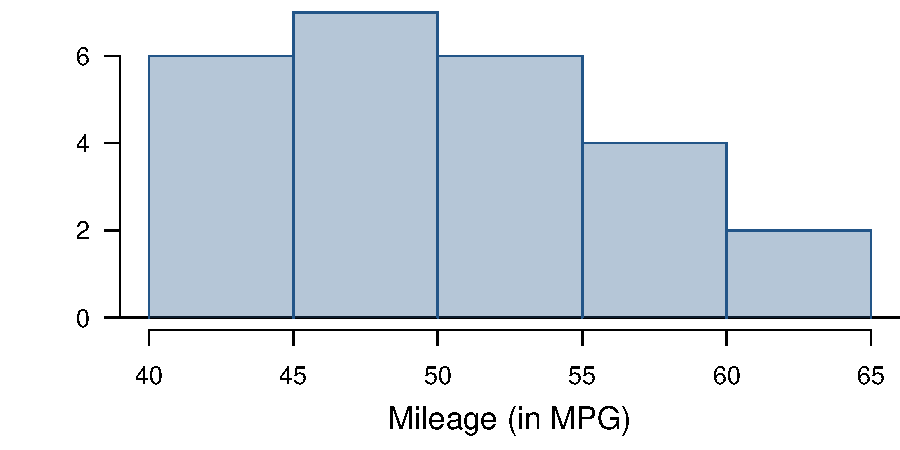
\includegraphics[width= \textwidth]{06/figures/eoce/prius09}
\end{center}
\end{minipage}
}
{
\begin{enumerate}[(a)]
\item This may not be reasonable since the sample may not be random. The drivers who volunteer to submit their gas mileage on fueleconomy.gov might be those that are getting much lower or much higher than the gas mileage estimated by the EPA.
\item The hypotheses are: $H_0: \mu = 46, H_A: \mu \ne 46$. \\
Before calculating the test statistic we should check that the assumptions and conditions are satisfied.
\begin{enumerate}[1.]
\item Independence assumption: 
\begin{itemize}
\item Randomization condition: We will assume that the sample is random though this assumption might not be plausible since drivers who volunteer to submit their gas mileage might be those that are getting much lower or much higher than the gas mileage claimed by the EPA.
\item 10\% Condition: 25 $<$ 10\% of all 2009 Prii.
\end{itemize}
Since we have a random sample and 10\% condition is met, we can assume that the gas mileage of one car in the sample is independent of another.
\item Nearly normal condition: The sample distribution looks somewhat right skewed but the skew is not very strong.
\end{enumerate}
The test statistic and the p-value can be calculated as follows:
\begin{align*}
T_{df} &= \frac{\bar{x} - \mu}{\frac{s}{\sqrt{n}}} = \frac{50.3 - 46}{\frac{6.8}{\sqrt{25}}} = 3.16 \\
df &= n - 1 = 25 - 1 = 24 \\
p-value < 0.01
\end{align*}
Since p-value $<$ 0.01 we reject $H_0$. The data provide strong evidence against the EPA claim of 46 MPG.
\item Given that $t_{24}^\star = 1.71$, a 90\% confidence interval can be calculated as follows:
\begin{align*}
\bar{x} \pm t_{df}^\star \frac{s}{\sqrt{n}} &= 50.3 \pm 1.71 \frac{6.8}{\sqrt{25}} \\
&= 50.3 \pm 2.3 \\
&= (48, 52.6)
\end{align*}
We are 90\% confident that a 2009 Prius gets on average 48 to 52.6 MPG.
\item Yes, we rejected $H_0$ and the interval does not include the null hypothesized value of 46 MPG.
\end{enumerate}
}
}

% 11

{\eoce{You are given the following hypotheses:
\begin{align*}
H_0&: \mu = 60 \\
H_A&: \mu < 60
\end{align*}
We know that the sample standard deviation is 8 and the sample size is 20. For what sample mean would the p-value be equal to 0.05? Assume that all assumptions and conditions necessary for inference are satisfied.
}
{
For the one-tailed p-value to be 0.05 at $n - 1 = 20 - 1 = 19$ degrees of freedom, T score needs to be -1.73. Then,
\[ -1.73 = \frac{\bar{x} - 60}{\frac{8}{\sqrt{20}}} \rightarrow \bar{x} = 56.91 \]
}
}

% 12

{\eoce{A 95\% confidence interval for a population mean, $\mu$, is given as (18.985, 21.015). This confidence interval is based on a simple random sample of 36 observations. Calculate the sample mean, $\bar{x}$, and the sample standard deviation, $s$. Assume that all assumptions and conditions necessary for inference are satisfied.}
{
The sample mean is the mid-point of the confidence interval, i.e. the average of the upper and lower bounds:
\[ \bar{x} = \frac{18.985 + 21.015}{2} = 20 \]
The margin of error is $21.015 - 20 = 1.015$. Since $n = 36$, $df = 35$, and the critical t-score is $t_{35}^\star = 2.03$. Then,
\[ 1.015 = 2.03 \frac{s}{\sqrt{36}} \rightarrow s = 3\]
}
}

%%%%%%%%%%%%%%%%%%%

\subsection{The t distribution for the difference of two means}

%%%%%%%%%%%%%%%%%%%

% 13

\eoce{Average income varies from one region of the country to another, and it often reflects both lifestyles and regional living expenses. Suppose a new graduate is considering a job in two locations, Cleveland, OH and Sacramento, CA, and she wants to see whether the average income in one of these cities is higher than the other. She would like to conduct a $t$ test based on two small samples from the 2000 Census, but she first must consider whether the conditions are met to implement the test. Below are a histograms for each city. Should she move forward with the $t$ test? Explain. \\
\begin{minipage}[c]{0.67\textwidth}
\begin{center}
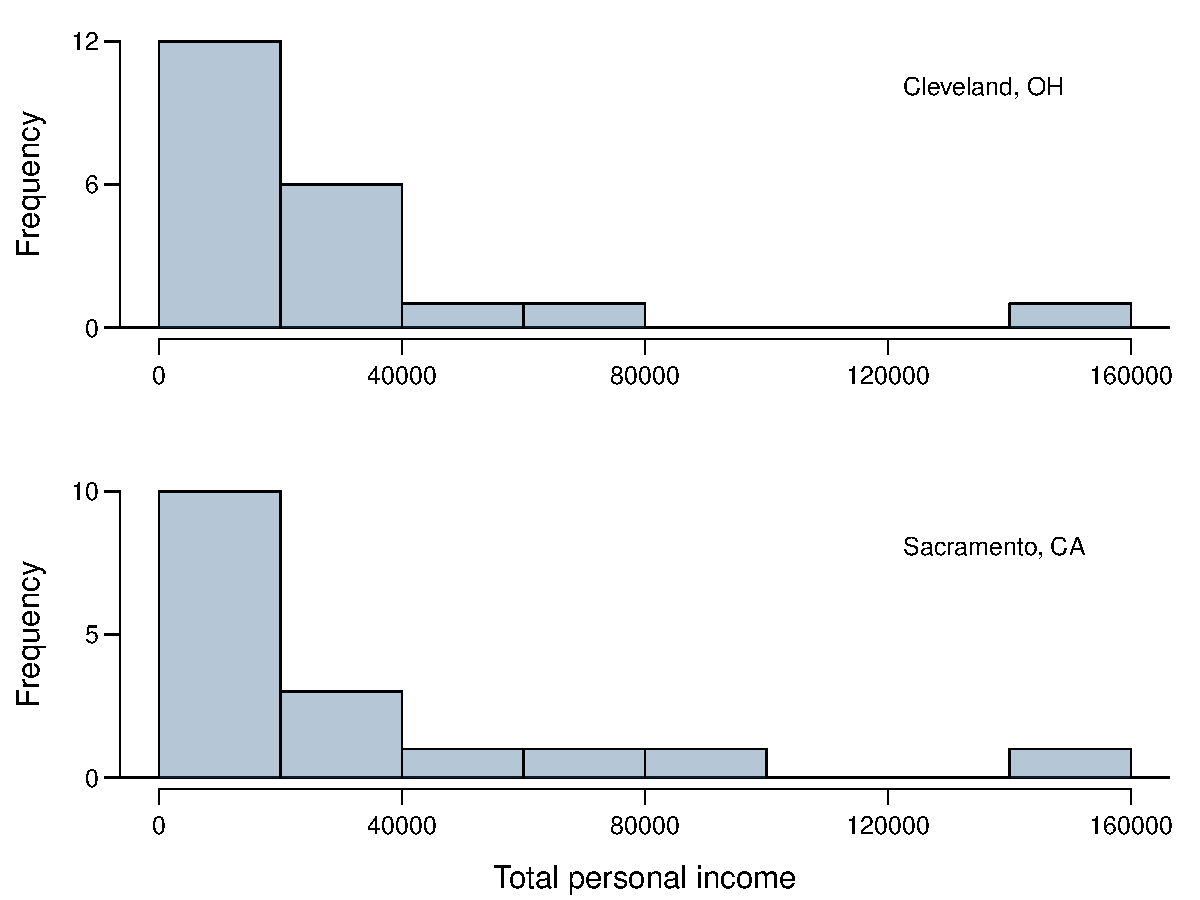
\includegraphics[width= \textwidth]{06/figures/eoce/incomeCleSac}
\end{center}
\end{minipage}
\begin{minipage}[c]{0.325\textwidth}
{\small
\begin{tabular}{l c}
\hline
		& Cleveland, OH	\\
\hline
Mean 	& \$ 26,436		\\
SD 		& \$ 33,239		\\
n 		& 21				
\end{tabular}

\vspace{2cm}

\begin{tabular}{l c}
\hline
		& Sacramento, CA \\
\hline
Mean	& \$ 32,182 \\
SD		& \$ 40,480 \\
n		& 17
\end{tabular}
}
\end{minipage}
}
{
No, a $t$ she should not move forward with the test since the distributions of total personal income are extremely skewed.
}

% 14

{\eoce{The first Oscar award for best actor and best actresses were given out in 1929. The histograms below show the age distribution for all the best actor and best actress winners from 1929 to 2011. Summary statistics for these distributions are also provided. Is a $t$ test appropriate for testing whether the difference in the sample means for age might be due to chance? Explain. \\
\begin{minipage}[c]{0.72\textwidth}
\begin{center}
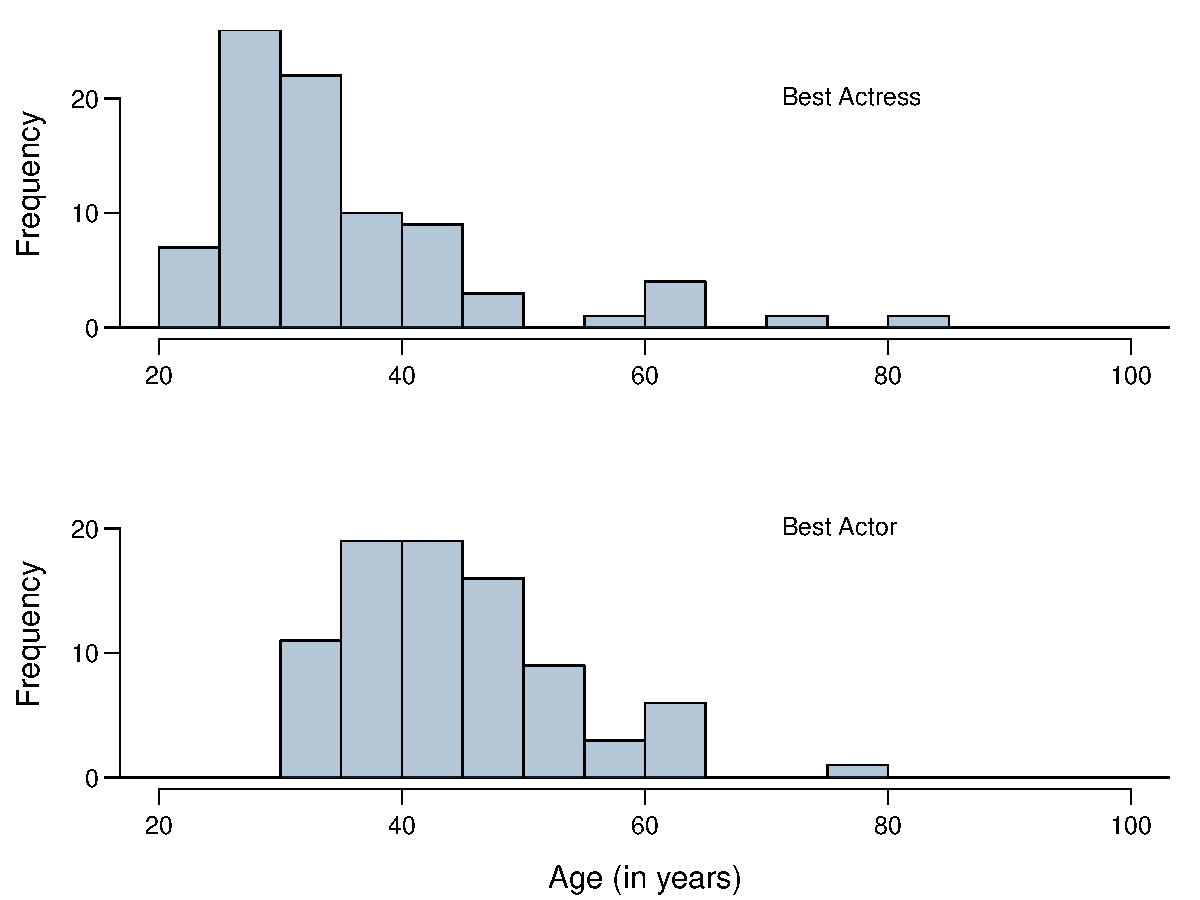
\includegraphics[width= \textwidth]{06/figures/eoce/oscarWinnersHist}
\end{center}
\end{minipage}
\begin{minipage}[c]{0.275\textwidth}
{\small
\begin{tabular}{l c}
\hline
		& Best Actress	\\
\hline
Mean 	& 35.6		\\
SD 		& 11.3		\\
n 		& 84				
\end{tabular}
$\:$ \\
\vspace{2cm}
$\:$ \\
\begin{tabular}{l c}
\hline
		& Best Actor \\
\hline
Mean	& 44.7 \\
SD		& 8.9 \\
n		& 84
\end{tabular}
}
\end{minipage}
}
{
These data come from a population (all oscar winners) not a random sample, so there is no need for hypothesis testing in this situation. We can see that the average age for the population of best actress winners is lower than the average age for the best actor winners.
}}


% 15

\eoce{Two independent random samples are selected from normal populations with unknown standard deviations. Both samples are small ($n < 50$). Find the p-value for the given set of hypotheses and $t$ values. Also determine if the null hypothesis would be rejected at $\alpha = 0.05$. Remember that a reasonable choice of degrees of freedom for the two-sample case is the minimum of $n_1-1$ and $n_2-1$. The ``exact" df is something we cannot compute from the given information.
\begin{enumerate}[(a)]
\setlength{\itemsep}{0mm}
\item $H_A: \mu_1 > \mu_2$, $n_1 = 23$, $n_2 = 25$, $T = 3.16$
\item $H_A: \mu_1 \ne \mu_2$, $n_1 = 38$, $n_2 = 37$, $T = 2.72$
\item $H_A: \mu_1 < \mu_2$, $n_1 = 45$, $n_2 = 41$, $T = -1.83$
\item $H_A: \mu_1 \ne \mu_2$, $n_1 = 11$, $n_2 = 15$, $T = 0.28$
\end{enumerate}
}
{
\begin{enumerate}[(a)]
\setlength{\itemsep}{0mm}
\item $H_A: \mu_1 > \mu_2$, $n_1 = 23$, $n_2 = 25$, $T = 3.16$, $df = min(23 - 1, 25 - 1) = min(22, 24) = 24$, $p-value < 0.005$, Reject $H_0$.
\item $H_A: \mu_1 \ne \mu_2$, $n_1 = 38$, $n_2 = 37$, $T = 2.70$, $df = min(38 - 1, 37 - 1) = min(37, 36) = 36$, p-value is about 0.01, Reject $H_0$.
\item $H_A: \mu_1 < \mu_2$, $n_1 = 45$, $n_2 = 41$, $T = -1.83$, $df = min(45 - 1, 41 - 1) = min(44, 40) = 40$, $0.025 < p-value < 0.05$, Reject $H_0$.
\item $H_A: \mu_1 \ne \mu_2$, $n_1 = 11$, $n_2 = 15$, $T = 0.28$, $df = min(11 - 1, 15 - 1) = min(10, 14) = 10$, $p-value > 0.20$, Fail to reject $H_0$.
\end{enumerate}
}

% 16

\eoce{Two independent random samples are selected from normal populations with unknown standard deviations. Both samples are small ($n < 50$). Find the degrees of freedom and the critical $t$ value ($t_{df}^\star$) for the given confidence level. \vspace{-2.5mm}
\begin{multicols}{2}
\begin{enumerate}[(a)]
\setlength{\itemsep}{0mm}
\item $n_1 = 16$, $n_2 = 16$, CL = 90\%. 
\item $n_1 = 36$, $n_2 = 41$, CL = 95\%
\item $n_1 = 8$, $n_2 = 10$, CL = 99\%
\item $n_1 = 23$, $n_2 = 27$, CL = 98\%
\end{enumerate}
\end{multicols}
}
{
\begin{enumerate}[(a)]
\setlength{\itemsep}{0mm}
\item $n_1 = 16$, $n_2 = 16$, CL = 90\%, $df = min(16 - 1, 16 - 1) = min(15, 15) = 15$, $t^{\star}_{15} = 1.75$
\item $n_1 = 36$, $n_2 = 41$, CL = 95\%, $df = min(36 - 1, 41 - 1) = min(35, 40) = 35$, $t^{\star}_{35} = 2.03$
\item $n_1 = 10$, $n_2 = 8$, CL = 99\%, $df = min(10 - 1, 8 - 1) = min(9, 7) = 7$, $t^{\star}_{7} = 3.50$
\item $n_1 = 23$, $n_2 = 27$, CL = 98\%, $df = min(23 - 1, 27 - 1) = min(22, 26) = 7$, $t^{\star}_{22} = 2.51$
\end{enumerate}
}

% 17

\eoce{A weight loss pill claims to accelerate weight loss when accompanied with exercise and diet. Diet researchers from a consumer advocacy group decided to test this claim using an experiment. 42 subjects were randomly assigned to two groups: 21 took the pill and 21 only received a placebo. Both groups underwent the same diet and exercise regiment. In the group that received the pill the average weight loss was 20\textit{lbs} with a standard deviation of 4\textit{lbs}. In the placebo group the average weight loss was 18\textit{lbs} with a standard deviation of 5\textit{lbs}. 
\begin{enumerate}[(a)]
\setlength{\itemsep}{0mm}
\item Calculate a 95\% confidence interval for the difference between the two means and interpret it in context.
\item Based on your confidence interval, is there significant evidence that the weight loss pill is effective?
\item Does this prove that the weight loss pill is effective?
\end{enumerate}
}
{
\begin{enumerate}[(a)]
\setlength{\itemsep}{0mm}
\item Before we can calculate the confidence interval, we need to find the degrees of freedom and $t^{\star}_{df}$.
\begin{align*}
df &= min(n_1 - 1, n_2 - 1) = min(20,20) = 20 \\
t^{\star}_{20} &= 2.09
\end{align*}
\begin{align*}
(\bar{x}_1 - \bar{x}_2) \pm t^{\star}_{df} \sqrt{\frac{s_1^2}{n_1} + \frac{s_2^2}{n_2}} &= (20 - 18) \pm 2.09 * \sqrt{\frac{4^2}{21} + \frac{5^2}{21}} \\
&= 2 \pm 2.92 \\
&= (-0.92, 4.92)
\end{align*}
We are 95\% confident that those in the group that got the weight loss pill lost 0.92\textit{lbs} less to 4.92\textit{lbs} more than those in the placebo group.

\item Since the confidence interval includes 0 there is no significant evidence that the weight loss pill is effective.

\item No, we can only say that the data \textit{suggest} that the pill is not effective, we did not prove that it is not. There may be other contributing factors. 
\end{enumerate}
}

% 18

\eoce{A company has two factories in which they manufacture engines. Once a month they randomly select 10 engines from each factory and test if there is a difference in performance in engines made in the two factories. This month the average output of the motors from Factory 1 is 120 horsepower with a standard deviation of 5 horsepower, and the average output of the motors from Factory 2 is 132 horsepower with a standard deviation of 4 horsepower. 
\begin{enumerate}[(a)]
\setlength{\itemsep}{0mm}
\item Calculate a 95\% confidence interval for the difference in the average horsepower for engines coming from the two factories and interpret it in context.
\item Based on your confidence interval, is there significant evidence that there is a difference in performance in engines made in the two factories? If so, can you tell which factory produces motors with lower performance? Explain.
\item Recently upgrades were made in Factory 2. Do these data prove that these upgrades enhanced the performance in engines made in this factory? Explain.
\end{enumerate}
}
{
\begin{enumerate}[(a)]
\setlength{\itemsep}{0mm}

\item Before we can calculate the confidence interval, we need to find the degrees of freedom and $t^{\star}_{df}$.
\begin{align*}
df &= min(n_1 - 1, n_2 - 1) = min(9,9) = 9 \\
t^{\star}_{9} &= 2.26
\end{align*}
\begin{align*}
(\bar{x}_1 - \bar{x}_2) \pm t^{\star}_{df} \sqrt{\frac{s_1^2}{n_1} + \frac{s_2^2}{n_2}} &= (120 - 132) \pm 2.26 * \sqrt{\frac{5^2}{10} + \frac{4^2}{10}} \\
&= -12 \pm 4.58 \\
&= (-16.58, -7.42)
\end{align*}
We are 95\% confident that average output of the motors made in Factory 1 is 7.42 to 16.58 horsepower lower than the motors made in Factory 2.

\item Yes, since the confidence interval does not include 0 there is significant evidence that there is a difference in performance in engines made in the two factories. Factory 1 produces motors with lower performance.

\item Even though there seems to be a statistically significant difference in the performances of engines made in the two factories, we can't tell if the upgrades made in Factory 2 \textit{caused} this. There may be other contributing factors.

\end{enumerate}
}

% 19

\eoce{Chicken farming is a multi-billion dollar industry, and any methods that increase the growth rate of young chicks can reduce consumer costs while increasing company profits, possibly by millions of dollars. An experiment was conducted to measure and compare the effectiveness of various feed supplements on the growth rate of chickens. Newly hatched chicks were randomly allocated into six groups, and each group was given a different feed supplement. Their weights in grams after six weeks are given along with feed types in the data set called \texttt{chickwts}. Below are some summary statistics from this data set along with box plots showing the distribution of weights by feed type. \citep{data:chickwts} \\
\noindent\begin{minipage}[c]{0.635\textwidth}
\begin{center}
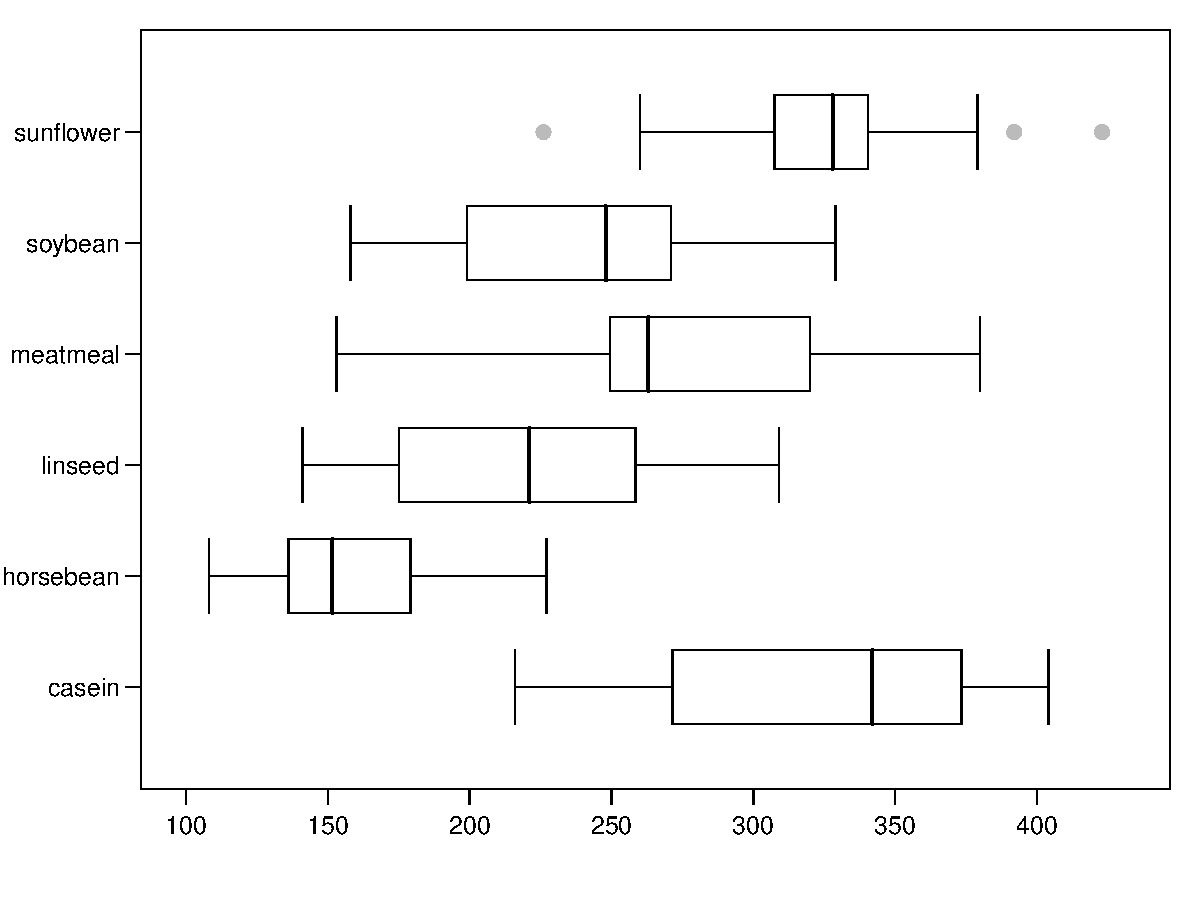
\includegraphics[width= \textwidth]{06/figures/eoce/chickwts.pdf}
\end{center}
\end{minipage}
\begin{minipage}[c]{0.36\textwidth}
{\footnotesize\begin{tabular}{l c c c}
\hline
       		& Mean		& SD		& n \\
\hline
casein  		& 323.58 		& 64.43	& 12 \\
horsebean 	& 160.20 		& 38.63	& 10 \\
linseed  		& 218.75 		& 52.24	& 12 \\
meatmeal 	& 276.91 		& 64.90	& 11 \\
soybean  		& 246.43 		& 54.13	& 14 \\
sunflower 		& 328.92 		& 48.84	& 12 \\
\hline
\end{tabular}}
\end{minipage} \vspace{-6mm}
\begin{enumerate}[(a)]
\setlength{\itemsep}{0mm}

\item Describe the distributions of weights of chickens that were fed linseed and horsebean.

\item Do these data provide strong evidence that the average weights of chicken that were fed linseed and horsebean are different? Use a 5\% significance level.

\item What type of error might we have committed? Explain.

\item Would your conclusion change if we used $\alpha = 0.01$?

\end{enumerate}
}
{
\begin{enumerate}[(a)]
\setlength{\itemsep}{0mm}

\item Chicken that were fed linseed on average weigh 218.75 grams while those that were given horsebean weigh on average 160.20 grams. Both distributions are relatively symmetric with no apparent outliers. There is a lot more variability in the weights of chicken that were given linseed.

\item Let linseed be group 1 and horsebean be group 2. Then,\\
$H_0: \mu_1 = \mu_2$ \\
$H_0: \mu_1 \ne \mu_2$ \\

Before calculating the test statistic we should check that the assumptions and conditions are satisfied.
\begin{enumerate}[1.]
\item Independence Assumption: 
\begin{itemize}
\item Random Sampling Condition: We are told that chickens are randomly assigned to feed groups.
\item 10\% Condition: 12 and 10 $<$ 10\% of all chickens fed linseed and horsebean.
\end{itemize}
Since we have random samples and the 10\% condition is satisfied for both samples, we can assume that the weights of chicken fed linseed are independent of each other, as well as the weights of chicken fed horsebean.
\item Nearly Normal Condition: We can see from the box plots that the distributions of weights of chicken in the two samples are pretty symmetric.
\item Independent Groups: Since assignment is done randomly the two samples are independent of each other.
\end{enumerate}

Since population standard deviations are unknown and samples are small we calculate a t score.

\[ T = \frac{(\bar{x}_1 - \bar{x_2}) - (\mu_1 - \mu_2)}{\sqrt{ \frac{s_1^2}{n_1} + \frac{s_2^2}{n_2} }} = \frac{(218.75 - 160.20) - 0}{ \sqrt{\frac{52.24^2}{12} + \frac{38.63^2}{10}} } = 3.02 \]
\[ df = min(n_1 - 1, n_2 - 1) = min(11,9) = 9 \]
\[ p-value = P(|t| > 3.02) \rightarrow 0.01 < p-value < 0.02 \]

Since p-value $<$ 0.05, we reject $H_0$. The data provide strong evidence that there is a significant difference between the average weights of chicken that were fed linseed and horsebean.

\item Type I, since we rejected $H_0$.

\item Yes, since p-value$> 0.01$, we would fail to reject $H_0$ and conclude that there isn't a significant difference between the average weights of chickens that were fed linseed and horsebean.

\end{enumerate}
}\label{chickwts}

% 20

\eoce{Casein is a common weight gain supplement for humans. Does it have the same effect on chickens? Using data provided in Exercise~\eoceref{chickwts}, test the hypothesis that the average weight of chickens that were fed casein is different than the average weight of chickens that were fed soybean. Assume that conditions for inference are satisfied.
}
{
Let casein be group 1 and soybean be group 2. Then,
$H_0: \mu_1 = \mu_2$ \\
$H_0: \mu_1 \ne \mu_2$ \\
\[ T = \frac{(\bar{x}_1 - \bar{x_2}) - (\mu_1 - \mu_2)}{\sqrt{ \frac{s_1^2}{n_1} + \frac{s_2^2}{n_2} }} = \frac{(323.58 - 246.43) - 0}{ \sqrt{\frac{64.43^2}{12} + \frac{54.13^2}{10}} } = 3.05 \]
\[ df = min(n_1 - 1, n_2 - 1) = min(11,13) = 11 \]
\[ p-value = P(t > 3.05) \rightarrow 0.01 < p-value < 0.02 \]
Since p-value $< \alpha$ (use $\alpha = 0.05$ since not given), reject $H_0$. The data provide strong evidence that the average weight of chickens that were fed casein is different than the average weight of chickens that were fed soybean.}

% 21

\eoce{Each year the US Environmental Protection Agency (EPA) releases fuel economy data on cars manufactured in that year. Below are summary statistics on fuel efficiency (in miles/gallon) from random samples of cars with manual and automatic transmissions manufactured in 2010. Do these data provide strong evidence of a difference between the average fuel efficiency of cars with manual and automatic transmissions in terms of their average city mileage? Assume that conditions for inference are satisfied. \citep{data:epaMPG2010} \vspace{-1.5mm}
\begin{center}
{\footnotesize\begin{tabular}{l c c c c c}
\hline
		& \multicolumn{2}{c}{City MPG}	& \multicolumn{2}{c}{Hwy MPG	} & \\
\hline
       		& Mean	& SD 	& Mean 	& SD 	& n \\
Manual  		& 21.08    		& 4.29    		& 29.31    		& 4.63 			& 26 \\
Automatic 	& 15.62    		& 2.76    		& 21.38    		& 3.73 			& 26 \\
\hline
\end{tabular}}
\end{center}
}
{
Let manual be group 1 and automatic be group 2. Then,
$H_0: \mu_1 = \mu_2$ \\
$H_0: \mu_1 \ne \mu_2$ \\
Since population standard deviations are unknown and samples are small we calculate a T score.

\[ t = \frac{(\bar{x}_1 - \bar{x_2}) - (\mu_1 - \mu_2)}{\sqrt{ \frac{s_1^2}{n_1} + \frac{s_2^2}{n_2} }} = \frac{(21.08 - 15.62) - 0}{ \sqrt{\frac{4.29^2}{26} + \frac{2.76^2}{26}} } = 5.46 \]
\[ df = min(n_1 - 1, n_2 - 1) = min(26 - 1, 26 - 1) = 25 \]
\[ p-value = P(|t| > 5.6) < 0.01 \]
Since p-value $< \alpha$ (use $\alpha = 0.05$ since not given), reject $H_0$. The data provide strong evidence that there is a significant difference in the average city mileage between cars with automatic and manual transmissions.}\label{epaMPG2010}

% 22

\eoce{An organization is studying whether women have caught up to men in starting pay after attending college. They randomly sampled 28 women, who earned an average of \$38,293.78 out of college with a standard deviation of \$5,170.22. Twenty-four men were also randomly sampled, and their earnings averaged \$41,981.82 with a standard deviation of \$3,195.42. Using a significance level of 0.02, do these data provide strong evidence that women have not yet caught up to men in terms of pay? If so, can we make a causal conclusion? If so, explain why. If not, provide an example of why the causal interpretation would not be valid. \\
}
{
Let women be group 1 and men be group 2. Then, \\
$H_0: \mu_{1} = \mu_{2}$, The average starting salaries for women and men are equal. \\
$H_A: \mu_{1} < \mu_{2}$, The average starting salaries for women and men are different. \\
Since population standard deviations are unknown and samples are small we calculate a T score.
\[ T = \frac{(\bar{x}_1 - \bar{x_2}) - (\mu_1 - \mu_2)}{\sqrt{ \frac{s_1^2}{n_1} + \frac{s_2^2}{n_2} }} = \frac{(38,293.78 - 41,981.82) - 0}{ \sqrt{\frac{5,170.22 ^2}{28} + \frac{3,195.42 ^2}{24}} } = -3.14 \]
\[ df = min(n_1 - 1, n_2 - 1) = min(28 - 1, 24 - 1) = 23 \]
\[ p-value < 0.005 \]
Since p-value $<$ 0.02, we reject $H_0$. The data provide strong evidence that women have not yet caught up to men in terms of pay. Since this is an observational study we cannot make a causal conclusion. There may be other lurking variables, such as the type of job women choose or can get after college.}
\label{menWomenSalaries}

% 23

\eoce{Exercise~\eoceref{epaMPG2010} provides data on fuel efficiency of cars manufactured in 2010. Use these statistics to calculate a 95\% confidence interval for the difference between average highway mileage of manual and automatic cars and interpret this interval in context.
}
{
\begin{align*}
df &= min(n_1 - 1, n_2 - 1) = min(26 - 1, 26 - 1) = 25 \\
t^{\star}_{25} &= 2.06
\end{align*}
\begin{align*}
(\bar{x}_1 - \bar{x}_2) \pm t^{\star}_{df} \sqrt{\frac{s_1^2}{n_1} + \frac{s_2^2}{n_2}} &= (29.31 - 21.38) \pm 2.06 * \sqrt{\frac{4.63^2}{26} + \frac{3.73^2}{26}} \\
&= 7.93 \pm 2.40 \\
&= (5.53, 10.33)
\end{align*}
We are 95\% confident that cars with manual transmission on average get 5.53 to 10.33 MPG more than cars with automatic transmission.
}

% 24

\eoce{Exercise~\eoceref{menWomenSalaries} provides summary statistics on the starting salaries of men and women who recently graduated from a college. Based on this information, calculate a 98\% confidence interval for the difference between the average starting salaries of such men and women and interpret this interval in context.
}
{
\begin{align*}
df &= min(n_1 - 1, n_2 - 1) = min(28 - 1, 24 - 1) = 23 \\
t^{\star}_{23} &= 2.50
\end{align*}
\begin{align*}
(\bar{x}_1 - \bar{x}_2) \pm t^{\star}_{df} \sqrt{\frac{s_1^2}{n_1} + \frac{s_2^2}{n_2}} &= (38,293.78 - 41,981.82) \pm 2.50 * \sqrt{\frac{5,170.22 ^2}{28} + \frac{3,195.42 ^2}{24}} \\
&= -3,688.04 \pm 1,174.79 \\
&= (2,513.25, 4,862.83)
\end{align*}
We are 98\% confident that men who recently graduated from Big Ten Universities with bachelor's degrees make \$2,513.25 to \$4,862.83 per year more than women with an equivalent educational background.
}

% 25

{\eoce{A group of researchers hypothesize that the presence of distracting stimuli during eating increases the meal size and could thereby contribute to overeating and obesity. To test their hypothesis, the researchers monitored food intake for a group of 44 patients who were randomized into two equal groups. The treatment group ate lunch while playing solitaire, and the control group ate lunch without any added distractions. Patients in the control group ate 57.1 grams of biscuits, with a standard deviation of 45.1 grams, and patients in the treatment group ate 27.1 grams of biscuits, with a standard deviation of 26.4 grams. Do these data provide strong evidence that the amount of biscuits consumed by the patients in the treatment and control groups are different? Assume that assumptions and conditions for inference are satisfied. \citep{Oldham:2011}
}
{
Let treatment be group 1 and control be group 2. Then, \\
$H_0: \mu_{1} = \mu_{2}$ \\
$H_A: \mu_{1} \ne \mu_{2}$. \\
Since population standard deviations are unknown and samples are small we calculate a T score.
\[ T = \frac{(\bar{x}_1 - \bar{x_2}) - (\mu_1 - \mu_2)}{\sqrt{ \frac{s_1^2}{n_1} + \frac{s_2^2}{n_2} }} = \frac{(57.1 - 27.1) - 0}{ \sqrt{\frac{45.1 ^2}{22} + \frac{26.4 ^2}{22}} } = 2.69 \]
\[ df = min(n_1 - 1, n_2 - 1) = min(22 - 1, 22 - 1) = 21 \]
\[ 0.01 < p-value < 0.02 \]
Since p-value $<$ 0.05, we reject $H_0$. The data provide strong evidence that the amount of biscuits consumed by the patients in the treatment and control groups are different.
}\label{solitaire}
}

% 26

{\eoce{The researchers from Exercise~\eoceref{solitaire} also investigated the effects of being distracted by a game on how much people eat. The 22 patients in the treatment group who ate their lunch while playing solitaire were asked to do a serial-order recall of the food lunch items they ate. The average number of items recalled by the patients in this group was 4.9, with a standard deviation of 1.8. The average number of items recalled by the patients in the control group (no distraction) was 6.1, with a standard deviation of 1.8. Do these data provide strong evidence that the average number of food items recalled by the patients in the treatment and control groups are different?}
{
Let treatment be group 1 and control be group 2. Then, \\
$H_0: \mu_{1} = \mu_{2}$ \\
$H_A: \mu_{1} \ne \mu_{2}$. \\
Since population standard deviations are unknown and samples are small we calculate a T score.
\[ T = \frac{(\bar{x}_1 - \bar{x_2}) - (\mu_1 - \mu_2)}{\sqrt{ \frac{s_1^2}{n_1} + \frac{s_2^2}{n_2} }} = \frac{(4.9 - 6.1) - 0}{ \sqrt{\frac{1.8 ^2}{22} + \frac{1.8 ^2}{22}} } = -2.21 \]
\[ df = min(n_1 - 1, n_2 - 1) = min(22 - 1, 22 - 1) = 21 \]
\[ 0.02 < p-value < 0.05 \]
Since p-value $<$ 0.05, we reject $H_0$. The data provide strong evidence that the average number of food items recalled by the patients in the treatment and control groups are different.
}
}

%%%%%%%%%%%%%%%%%%%

\subsection{Small sample hypothesis testing for a proportion}

%%%%%%%%%%%%%%%%%%%

% 27

\eoce{A popular uprising that started on January 25, 2011 in Egypt led to the 2011 Egyptian Revolution. Polls show that about 69\% of American adults followed the news about the political crisis and demonstrations in Egypt closely during the first couple weeks following the start of the uprising. Among a random sample of 30 high school students, it was found that only 17 of them followed the news about Egypt closely during this time. \citep{web:egypt}
\begin{enumerate}[(a)]
\setlength{\itemsep}{0mm}
\item Write the hypotheses for testing if the proportion of high school students who followed the news about Egypt is different than the proportion of American adults who did.
\item Calculate the proportion of high schoolers in this sample who followed the news about Egypt closely during this time.
\item For large sample theory, we modeled $\hat{p}$ using the normal distribution. Why should we be cautious about this approach for these data?
\item Since the normal approximation may not be as reliable here as a small sample approach, we evaluate the hypotheses using a simulation. Describe how to perform such a simulation and, once you had results, how to estimate the p-value.
\item Below is a histogram showing the distribution of $\hat{p}_{sim}$ in 10,000 simulations under the null hypothesis. Estimate the p-value using the plot and determine the conclusion of the hypothesis test.
\begin{center}
\includegraphics[width=0.8\textwidth]{06/figures/eoce/egypt}
\end{center}
\end{enumerate}
}
{
\begin{enumerate}[(a)]
\setlength{\itemsep}{0mm}
\item $H_0: p = 0.69$ \\
$H_A: p \ne 0.69$
\item $\hat{p} = \frac{17}{30} = 0.57$
\item The success-failure condition is not satisfied. Under the null hypothesis, we would expect to have 30*0.69 = 20.7 high school students to follow the news and 30*0.31 = 9.3 to not follow the news, not the 10 required for the normal approximation.
\item Each student can be represented with a card. Take 100 cards, 69 black cards representing those who follow the news about Egypt and 31 red cards representing those who do not. Shuffle the cards and draw with replacement 30 cards representing the 30 high school students. Calculate the proportion of black cards in this sample, $\hat{p}_{sim}$, i.e. the proportion of those who follow the news. Repeat 10,000 times and plot the resulting sample proportions. The p-value will be two times the proportion of simulations where $\hat{p}_{sim} \le 0.57$.
\item The p-value is represented by the area shown below in blue. In 1,348 out of the 10,000 $\hat{p}_{sim} \le 0.57$, therefore p-value $= 2 * \frac{1348}{10000} = 0.2696$. (Note that students may have approximate results.) 
\noindent \begin{minipage}[c]{0.5\textwidth}
Since p-value is high, we fail to reject $H_0$. The data do not provide strong evidence that the proportion of high school students who followed the news about Egypt is lower than the proportion of American adults who did. 
\end{minipage}
\begin{minipage}[c]{0.5\textwidth}
\begin{center}
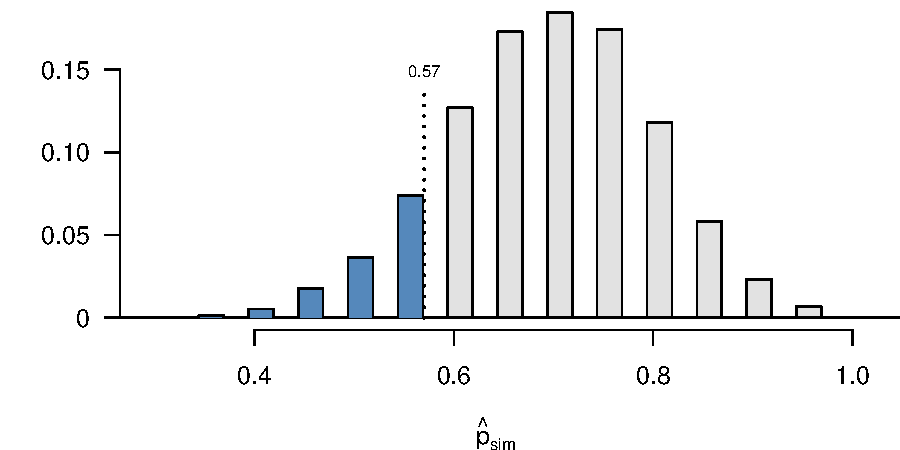
\includegraphics[width= 0.9\textwidth]{06/figures/eoce/egyptSoln}
\end{center}
\end{minipage}
\end{enumerate}
}

% 28

\eoce{Assisted Reproductive Technology (ART) is a collection of techniques that help facilitate pregnancy (e.g. in vitro fertilization). A 2008 report by the Centers for Disease Control and Prevention estimated that ART has been successful in leading to a live birth in 31\% of cases \citep{web:art}. A new infertility clinic claims that their success rate is higher than average. A random sample of 30 of their patients yielded a success rate of 40\%.
\begin{enumerate}[(a)]
\setlength{\itemsep}{0mm}
\item Write the hypotheses to test if the success rate for ART at this clinic is significantly higher than the average success rate.
\item For large sample theory, we modeled $\hat{p}$ using the normal distribution. Why is this not appropriate here?
\item The normal approximation would be less reliable here, so we use a simulation strategy. Describe a setup for a simulation that would be appropriate in this situation and how the p-value can be calculated using the simulation results.
\item Below is a histogram showing the distribution of $\hat{p}_{sim}$ in 10,000 simulations under the null hypothesis. Estimate the p-value using the plot and use it to evaluate the hypotheses.
\begin{center}
\includegraphics[width=0.8\textwidth]{06/figures/eoce/art}
\end{center}
\end{enumerate}
}
{
\begin{enumerate}[(a)]
\setlength{\itemsep}{0mm}
\item $H_0: p = 0.31$ \\
$H_A: p > 0.31$
\item The success-failure condition is not satisfied. Under the null hypothesis, we would expect to have 25*0.31 = 7.75 
live births, not the 10 required for the normal approximation.
\item Each patient can be represented with a card. Take 100 cards, 31 black cards representing successful ART cycles and 69 red cards representing unsuccessful ART cycles. Shuffle the cards and draw with replacement 25 cards representing these patients. Calculate the proportion of black cards in this sample, $\hat{p}_{sim}$, i.e. the proportion of successful ART cycles. Repeat 10,000 times and plot the resulting sample proportions. The p-value will be the proportion of simulations where $\hat{p}_{sim} \ge 0.40$.
\item The p-value is represented by the area shown below in blue. In 2,285out of the 10,000 $\hat{p}_{sim} > 0.40$, therefore p-value $= \frac{1158}{10000} = 0.2285$. (Note that students may have approximate results.) 
\noindent \begin{minipage}[c]{0.5\textwidth}
Since p-value is high, we fail to reject $H_0$. The data do not provide strong evidence that the the success rate for ART at this clinic is significantly higher than the average success rate.
\end{minipage}
\begin{minipage}[c]{0.5\textwidth}
\begin{center}
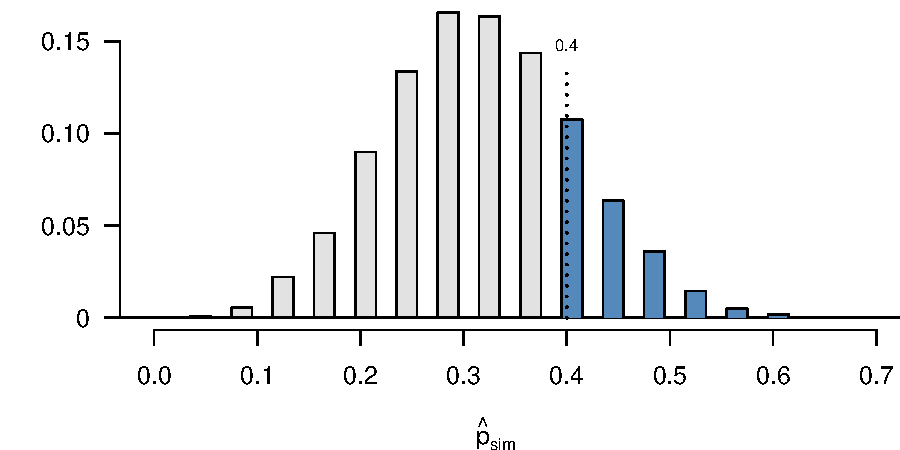
\includegraphics[width= 0.9\textwidth]{06/figures/eoce/artSoln}
\end{center}
\end{minipage}
\end{enumerate}
}

%%%%%%%%%%%%%%%%%%%

\subsection{Hypothesis testing for two proportions}

%%%%%%%%%%%%%%%%%%%

% 29

\eoce{A ``social experiment" conducted by a TV program questioned what people do when they see a very obviously bruised woman getting picked on by her boyfriend. On two different occasions at the same restaurant the same couple was depicted, however in one scenario the woman was dressed ``provocatively" and in the other scenario the woman was dressed ``conservatively". The table below shows how many restaurant diners were present under each scenario, and whether or not they intervened.
\begin{center}
\begin{tabular}{ll cc c} 
			&				& \multicolumn{2}{c}{\textit{Scenario}} \\
\cline{3-4}
							&			& Provocative	& Conservative 	& Total	\\
\cline{2-5}
\multirow{2}{*}{\textit{Intervene}}	&Yes 		& 5	 	& 15		& 20 	\\
							&No			& 15	 	& 10 	 	& 25 \\
\cline{2-5}
							&Total		& 20		& 25		& 45 \\
\end{tabular}
\end{center}
A simulation was conducted to test if people react differently under the two scenarios. In order to conduct the simulation, a researcher wrote yes on 20 index cards and no on 25 index cards to indicate whether or not a diner (represented by each card) intervened. Then he shuffled the cards and dealt them into two groups of size 20 and 25, the provocative and conservative scenarios, respectively. He counted how many diners in each scenario intervened, calculated the difference between the simulated proportions of intervention as $\hat{p}_{pr,sim} - \hat{p}_{con,sim}$. This simulation was repeated 10,000 times using software to obtain 10,000 differences that are due to chance alone. The histogram below shows the distribution of the simulated differences.
\begin{center}
\includegraphics[width=0.8\textwidth]{06/figures/eoce/socExp}
\end{center}
\begin{enumerate}[(a)]
\setlength{\itemsep}{0mm}
\item What are the hypotheses?
\item Calculate the observed difference between the rates of intervention under the two scenarios.
\item Estimate the p-value using the figure above and determine the conclusion of the hypothesis test.
\end{enumerate}
}
{
\begin{enumerate}[(a)]
\setlength{\itemsep}{0mm}
\item $H_0: p_{provocative} = p_{conservative}$ \\
$H_A: p_{provocative} \ne p_{conservative}$
\item $\frac{5}{20} - \frac{15}{25} = -0.35$
\item The p-value is represented by the area shown below in blue. In 143 out of the 10,000 simulations differences under the null hypothesis was less than or equal to 0.35. Doubling the one tail, the p-value is about 0.03. (Note that students may have approximate results.)

\noindent \begin{minipage}[c]{0.5\textwidth}
Since p-value is low, we reject $H_0$. The data provide strong evidence that people react differently under the two scenarios.
\end{minipage}
\begin{minipage}[c]{0.5\textwidth}
\begin{center}
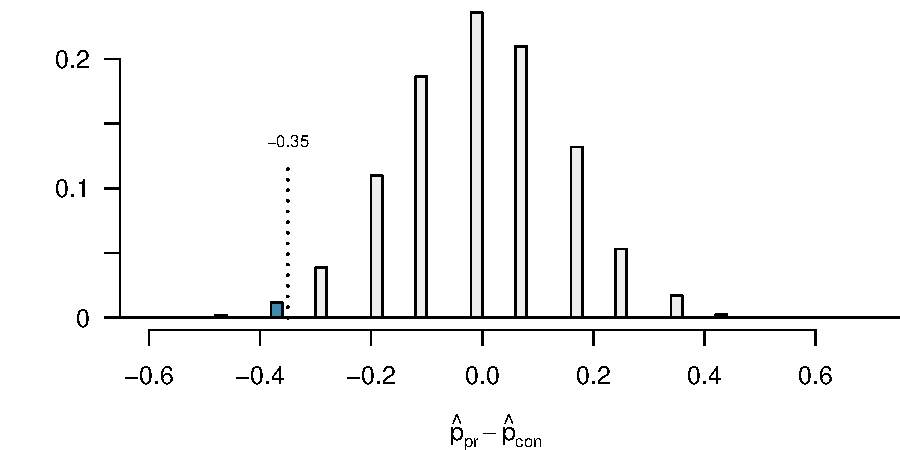
\includegraphics[width= 0.9\textwidth]{06/figures/eoce/socExpSoln}
\end{center}
\end{minipage}
\end{enumerate}
}

% 30

{\eoce{An experiment conducted by the \textit{MythBusters}, a science entertainment TV program on the Discovery Channel, tested if a person can be subconsciously influenced into yawning if another person near them yawns. 50 people were randomly assigned to two groups: 34 to a group where a person near them yawned (treatment) and 16 to a group where there wasn't a yawn seed (control). The following table shows the results of this experiment. \citep{data:yawn}
\begin{center}
\begin{tabular}{ll cc c} 
			&				& \multicolumn{2}{c}{\textit{Group}} \\
\cline{3-4}
							&			& Treatment	& Control 	& Total	\\
\cline{2-5}
\multirow{2}{*}{\textit{Result}}		&Yawn 		& 10	 	& 4		& 14 	\\
							&Not Yawn	& 24	 	& 12 	 	& 36 \\
\cline{2-5}
							&Total		& 34		& 16		& 50 \\
\end{tabular}
\end{center}
A simulation was conducted to test if people are more likely to yawn if a person near them yawns. In order to conduct the simulation, a researcher wrote yawn on 14 index cards and not yawn on 36 index cards to indicate whether or not a person yawned. Then he shuffled the cards and dealt them into two groups of size 34 and 16, for treatment and control, respectively. He counted how many participants in each group yawned in an apparent response to a nearby yawning person, calculated the difference between the simulated proportions of yawning as $\hat{p}_{trtmt,sim} - \hat{p}_{ctrl,sim}$. This simulation was repeated 10,000 times using software to obtain 10,000 differences that are due to chance alone. The histogram below shows the distribution of the simulated differences.
\begin{center}
\includegraphics[width=0.8\textwidth]{06/figures/eoce/yawn}
\end{center}
\begin{enumerate}[(a)]
\setlength{\itemsep}{0mm}
\item What are the hypotheses?
\item Calculate the observed difference between the yawning rates under the two scenarios.
\item Estimate the p-value using the figure above and determine the conclusion of the hypothesis test.
\end{enumerate}
}
{
\begin{enumerate}[(a)]
\setlength{\itemsep}{0mm}
\item $H_0: p_{treatment} = p_{control}$ \\
$H_A: p_{treatment} > p_{control}$
\item $\frac{10}{34} - \frac{4}{16} = 0.04$
\item The p-value is represented by the area shown below in blue. In 4879 out of the 10,000 simulations differences under the null hypothesis was greater than or equal to 0.04. Therefore the p-value is 0.4879. (Note that students may have approximate results.) \\
\noindent \begin{minipage}[c]{0.5\textwidth}
Since p-value is high, we fail to reject $H_0$. The data do not provide strong evidence that people are more likely to yawn if a person near them yawns
\end{minipage}
\begin{minipage}[c]{0.5\textwidth}
\begin{center}
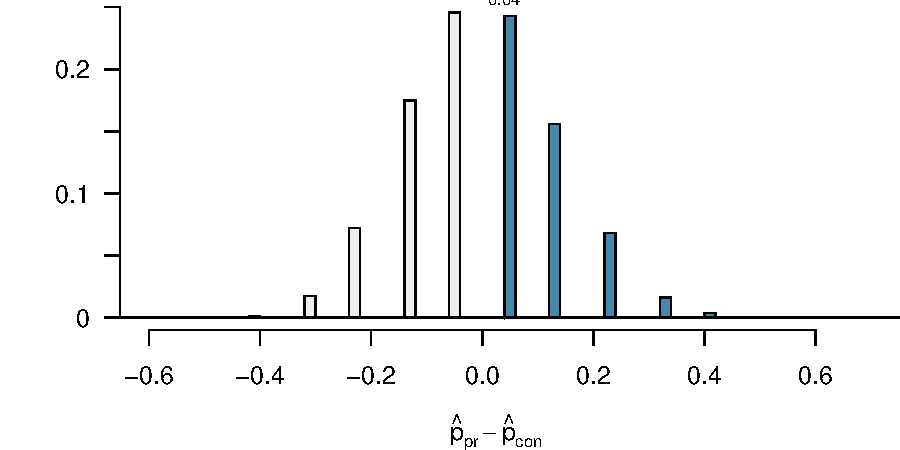
\includegraphics[width= 0.9\textwidth]{06/figures/eoce/yawnSoln}
\end{center}
\end{minipage}
\end{enumerate}
}
}



%%%%

%\bibliographystyle{ieeetr}
%\bibliography{chp6ex}	
